\documentclass[12pt]{article}
\usepackage[top=1in, bottom=1in, left=1in, right=1in]{geometry}
%\usepackage[margin=1in]{geometry}
\usepackage[onehalfspacing]{setspace}
%\usepackage[doublespacing]{setspace}
\usepackage{amsmath, amssymb, amsthm}
\usepackage{enumerate, enumitem}
\usepackage{fancyhdr, graphicx, proof, comment, multicol}
\usepackage[none]{hyphenat} % This command prevents hyphenation of words
\binoppenalty=\maxdimen % This command and the next prevent in-line equation breaks
\relpenalty=\maxdimen
%    Good website with common symbols
% http://www.artofproblemsolving.com/wiki/index.php/LaTeX%3ASymbols
%    How to change enumeration using enumitem package
% http://tex.stackexchange.com/questions/129951/enumerate-tag-using-the-alphabet-instead-of-numbers
%    Quick post on headers
% http://timmurphy.org/2010/08/07/headers-and-footers-in-latex-using-fancyhdr/
%    Info on alignat
% http://tex.stackexchange.com/questions/229799/align-words-next-to-the-numbering
% http://tex.stackexchange.com/questions/43102/how-to-subtract-two-equations
%    Text align left-center-right
% http://tex.stackexchange.com/questions/55472/how-to-make-text-aligned-left-center-right-in-the-same-line
\usepackage{microtype} % Modifies spacing between letters and words
\usepackage{mathpazo} % Modifies font. Optional package.
\usepackage{mdframed} % Required for boxed problems.
\usepackage{parskip} % Left justifies new paragraphs.
\linespread{1.1} 


%figure support
\usepackage{import}
\usepackage{xifthen}
\pdfminorversion=7
\usepackage{pdfpages}
\usepackage{transparent}
\newcommand{\incfig}[1]{%
	\def\svgwidth{\columnwidth}
	\import{./figures/}{#1.pdf_tex}
}
\graphicspath{ {./figures/} }
\pdfsuppresswarningpagegroup=1

\newenvironment{problem}[1]
{\begin{mdframed}[linewidth=0.6pt]
        \textsc{Problem #1:}

}
    {\end{mdframed}}

\newenvironment{solution}
    {\textsc{Solution:}\\}
    {\newpage}% puts a new page after the solution
    
\newenvironment{statement}[1]
{\begin{mdframed}[linewidth=0.6pt]
        \textsc{Statement #1:}

}
    {\end{mdframed}}

\newenvironment{prf}
   {\textsc{Proof:}\\}
   {\newpage}% puts a new page after the solution

\begin{document}
% This is the Header
% Make sure you update this information!!!!
\noindent
\textbf{COP4610.01} \hfill \textbf{Brandon Thompson} \
\normalsize Prof. Jaimes \hfill Due Date: 1/23/20 \

% This is where you name your homework
\begin{center}
\textbf{Programming Assignment 1}
\end{center}
	\subsubsection*{Deliveries:}
	\begin{itemize}
		\item \textbf{Code:} a .c program following the problem statement.
		\item \textbf{Report:} Brief report explaining how you address
			the problem, and screenshots of the output.
	\end{itemize}
	\textbf{Requirements:} The program should use the POSIX api from unix/linux,
	and should run in the university UNIX system (ember).\\
	\textbf{Note:} Use your student ID number as your program name.\\
	\hline
	I certify that I coded this program by myself and this code doesn't correspond
	to the intellectual work of someone else.\\\\
	\begin{tabular}{@{}p{.5in}p{4in}@{}}
		Signature:  & \ \ \hrulefill \\
	\end{tabular}

	\subsubsection*{Problem} 
	Write a program that takes integer $n$ and a list of integers $A$ where
	size of $A$ is a multiple of $n$ where $n \le 10$ and $n$ is the number of children
	to create. Each child will compute the sum of subarray $a \in A$ and
	return the partial sum to the parent. Parent will print the total sum.
	\clearpage	
	\subsubsection*{Steps}
        \begin{enumerate}
		\item Verify that size of $A$ is a multiple of  $n$. 
		\item Pull arguments from argument list \verb|char *argv[]|.
		\item Split $A$ into $n$ subarrays.
		\item Initialize communication between processes with pipes,
			\verb|p[childNum][P/C][R/W]|.
		\item Pass $a$ from parent to child.
		\item Child returns partial sum to parent.
		\item Parent adds partial sum to final sum.
		\item Repeat steps 5,6,7 for each child.
		\item Parent prints final sum.
        \end{enumerate}
	\begin{figure}[ht!]
		\centering
		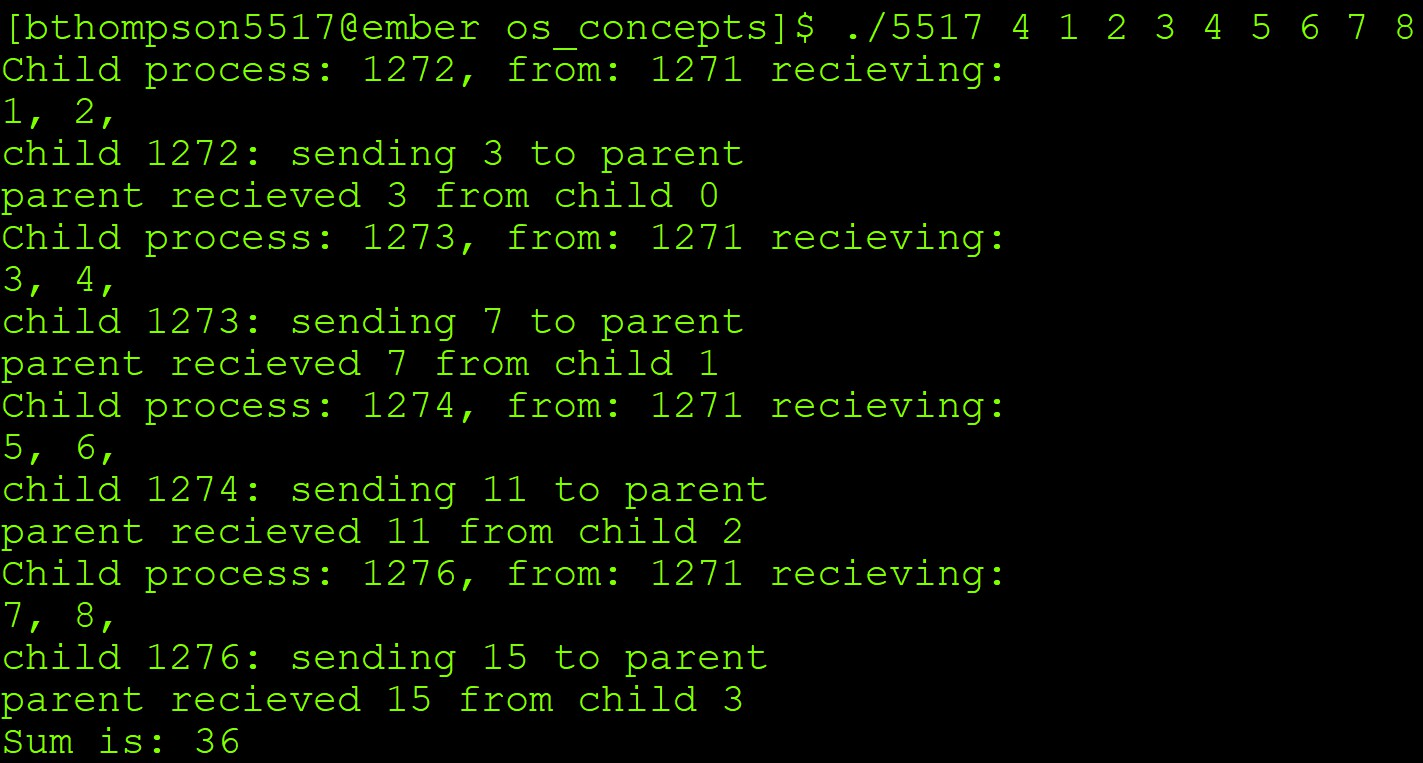
\includegraphics[width=0.9\textwidth]{assignment1.jpg}
		\caption{Screenshot of program creating 4 children.}
		\label{fig:assignment1}
	\end{figure}
\end{document}
